\section{Calculation of vibrational and phonon frequencies}
\label{Sec:vib}

There are two separate script-based tools in the FHI-aims code that
can be used to obtain vibrational frequencies for molecules and
clusters as well as phonons for periodic systems. These analyses
are always based on finite-difference calculations of a converged
structure. Both tools have the form of a \option{perl}-script wrapper, 
which does all necessary DFT calculations and then calls a routine 
to set up and diagonalize the Hessian matrices.

To compile the tools, change into the source directory from which you
also compiled the original FHI-aims. With the same Makefile settings
as for the main program, type either 

\option{make vibrations}

or

\option{make vibrations.mpi}.

The make targets for the phonons are \option{phonons} and
\option{phonons.mpi}. It is recommended that MPI-routines are compiled
into these binaries whenever an MPI version of the code is being
used. 

These Make targets will create two files in the FHI-aims binary
directory. One is the actual diagonalization subprogram, the other one
the \option{perl}-wrapper. \textbf{You will need to edit the header of the
\option{perl}-wrapper scripts} and give three key parameters: The
absolute location of the FHI-aims binary directory
(\option{\$AIMS\_BINDIR}), the aims executable to be used
(\option{\$EXE}), and the calling command for the executable 
(\option{\$CALLING\_PREFIX} and \option{\$CALLING\_SUFFIX}).
The \option{\$CALLING\_PREFIX} is required for specification of
parallel runs, for example 

\option{\$CALLING\_PREFIX = mpirun -np 2}

for a two-core parallel run. In addition, some parallel environments
(most notably IBM's \option{poe} require that the number of cores is
specified after the executable is called, for those instances you can
set \option{\$CALLING\_PREFIX}. Note that the postprocessing routines
for both, the vibrations and the phonons are also
parallel. Specifically, the calculation of the phonon density of
states makes good use of that functionality. 

Having compiled the vibrations and/or phonon scripts, running them is
very simple and will be demonstrated by two examples. Both are
provided with the code distribution.

\subsection*{Vibrations of a water molecule}

We use the same water molecule that was relaxed in the example section
\ref{Sec:example-Etot}. This test case is
contained in the directory \option{testrun/H2O-vibrations}.

The vibrational frequencies are very sensitive to the residual forces on the relaxed
molecular geometry, as well as they have a very strong dependence on
the accuracy of the forces. Remember, we are trying to calculate a
second derivative of the energy from the numerical derivative on the
forces arising from small finite displacements. In order to avoid
problems arising from this complication, we apply the following
changes to the original \option{control.in}:
\begin{itemize}
\item use the exact species defaults for elements H and O, up to
  tier2. This includes slightly denser grids than were used for the
  relaxation and leads to more accurate forces
\item increase the force accuracy \keyword{sc\_accuracy\_forces} to
  \option{1E-5}
\item change the \keyword{relax\_geometry} \option{bfgs} to \option{1E-3}.
\end{itemize}
These new settings contain all that is necessary to get close enough
to the actual minimum 
Note that the total energy of the structure basically does not change
throughout a post-relaxation (meaning that the original relaxation
criterion was quite good enough), but that the purpose of this
exercise has to be to get very close to the actual minimum for
accurate vibrations. 

In order to run the vibrations, change to the directory containing the
input files and run the aims.vibration.* script in the
directory. That's it. The calculation should take no more than a few
minutes to complete, it first relaxes the structure to its minimum
configuration and then applies six finite displacements to each of the
atoms - 18 single-point calculations in total for the water
molecule. 

The output stream contains all of the important data, which is
additionally saved in a number of temporary and output files. The file
basic.vib.out contains the output of the normal mode
analysis, while the file basic.xyz contains the actual eigenmodes
(vibrations), which can be read by a number of molecular viewers. 

If you did your calculations as described here, the vibration script
automatically assumes a jobname \option{basic}, which can also be
changed by adding it to the vibration script, which has the following
complete calling form:
\option{aims.vibrations.version.pl jobname delta}

This syntax requires your original control files to have the
name \option{control.in.\$jobname} and \option{geometry.in.\$jobname}.
The second possible parameter, \option{delta}, is the finite
displacement used for calculating the Hessian matrix. Its default is
0.001 \AA, which has been doing a good job for all the cases we are
aware of, but it is somewhat smaller than the values one generally
encounters in the literature. Please verify that it works for your
application if you have any doubts. 

Finally, a short note on the actual physical output basic.vib.out: Given are the
frequencies in cm$^{1}$, the corresponding zero point energies in eV,
and their cumulative total. It is vital to ensure that the first six
eigenmodes are zero, which means that the structure in question
actually corresponds to a minimum on the potential energy surface. 
FHI-aims does no explicit reduction of the translational and
rotational eigenmodes, which allows an explicit check on the quality
of the strucure.

In the example provided, the \emph{first} mode has a frequency of
-7 cm$^{-1}$, which could be reduced to -5 cm$^{-1}$ when the BFGS
convergence criteron is set to 1E-5. However, since the first actual
vibration is at 1593 cm$^{-1}$, there is no need to worry about this
fact. 

\subsection*{Phonon calculations in general}

To obtain proper phonon spectra some extra information is
necessary. To calculate the phonons, we use the so-called
\emph{direct} or \emph{supercell} method, based on the approximations
that the interactions necessary to calculate the phonons are
finite [see e.g. Ref. \cite{Parlinski97} and references therein
for details of the method]. All phonon related functionality is driven
with a single keyword \keyword{phonon}, specified in the
\option{control.in}. Its various instances and options are described
in this section. 

The phonon calculation proceeds as follows. A single (user-specified) unit cell is
extended a number of times in the direction of all three basis
vectors. A finite displacement technique as in the vibrations is then
used to gather the necessary force response, which then makes up a
basic force constant matrix. All finite displacement structures are
investigated for their symmetry (within the octahedral group), such as
to minimize the computations required and also to obtain properly
symmetrized forces where applicable. Finally, the force constant matrix is
diagonalized for a number of selected reciprocal lattice points
(i.e. along the requested bands) and the eigenvalues give the phonon
spectra. Two things are absolutely vital:
\begin{itemize}
\item {\bf converge your supercell size!} The minimum sensible cell
  is $2\times 2\times 2$, and it might be tempting to restrict a
  calculation to this size, but it will be almost certainly wrong for
  small unit cell sizes, as shown in the example below.
\item {\bf the geometry.in MUST contain only the primitive 1x1x1 cell
  of your lattice!}. The phonon calculation copies its own
  supercell. If, by accident, your \option{geometry.in} already
  contains a $3\times3\times3$ supercell and you request phonons for a $3\times3\times3$
  supercell on top of that, you will end up with a
  $(3\times3\times3)^2=729$ atom calculation, which will almost
  certainly be too much for your computer... 
\end{itemize}
The phonon script is invoked from a directory containing a
\option{control.in} and a \option{geometry.in} file. As there are a
number of working files involved in the calculation, a directory
\option{phonon\_workdir} is made in which all DFT calculations are
done and where the postprocessing happens. The advantage of such an
approach is that the script can be stopped at any time without losing
any information at all. In fact, once the DFT results are present, the
entire script can be rerun multiple times to optimize the phonon
output without having to redo the expensive DFT analysis over again. 
All the physical output is given either in standard out or as files
in the directory from which the phonon script was invoked. 

Without much further ado, here is the description of the commands
required to calculate lattice vibrations:

\keydefinition{phonon}{control.in}
{
  Usage: \keyword{phonon} \option{[subkeywords and their options]}\\[1.0em]
  Purpose: Main driver keyword for the phonon calculation script. has
  the subkeywords \subkeyword{phonon}{supercell},
  \subkeyword{phonon}{band}, \subkeyword{phonon}{dos},
  \subkeyword{phonon}{displacement}, as detailed below.\\ }

\subkeydefinition{phonon}{band}{control.in}
{ Usage: \keyword{phonon} \subkeyword{phonon}{band} \option{kstart1
    kstart2 kstart3 kend1 kend2 kend3 npoints startname endname} \\[1.0em]
  Purpose: To define a phonon band to be plotted explicitly. The
  remaining syntax is kept the same as for the \keyword{output} option
  \subkeyword{output}{band}: the first six parameters describe the
  starting and ending point in RELATIVE \emph{k}-coordinates,
  \option{npoints} is the number of points in the band, followed by
  the names of the special points for starting and ending the band. \\}
As for the band structure output (see also section \ref{band and dos plotting}), 
there is no real need for naming the special points as far as FHI-aims
or the phonon calculation is concerned, but we provide a translator
script for the output, which then plots a 'nice' phonon band structure
on a single axis and uses the names of these points. 

\subkeydefinition{phonon}{displacement}{control.in}
{ Usage: \keyword{phonon} \subkeyword{phonon}{displacement}
  \option{delta} \\[1.0em]
  Purpose: To define the absolute displacement of each atom for the
  finite difference calculation. \\[1.0em]
  Default: 0.001 \AA\\}

\subkeydefinition{phonon}{dos}{control.in}
{ Usage: \keyword{phonon} \subkeyword{phonon}{dos} \option{fstart fend
  fpoints broad qdensity}\\[1.0em]
  Purpose: governs the output of the phonon density of states. \\ }
This keyword produces a DOS output to the file
\option{phonon\_dos.dat}, which describes the DOS along a frequency
axis in THz. \option{fstart}, \option{fend}, and \option{broad} give
the starting and ending frequency as well as the broadening in units
of THz, while \option{fpoints} is the number of points. Unlike the
output option \subkeyword{output}{dos}, here we also have to specify a
$k$-point density \option{qdensity}, which does the BZ integration on
a \option{qdensity}$\times$\option{qdensity}$\times$\option{qdensity}
grid. Normally, the dynamic matrix only contains a very small number
of elements (3 in the example described below), which means that one
can chose \option{qdensity} quite high in order to get a
well-converged density of states. Notice that this value might be changed by the program
if the DOS and $c_v$ calculations are requested at the same time. In
that case, the higher of the two values for \option{qdensity}
specified for the two calculations is chosen in order to minimize the
computational effort. See also the \subkeyword{phonon}{free\_energy}
description. 

\subkeydefinition{phonon}{free\_energy}{control.in}
{ Usage: \keyword{phonon} \subkeyword{phonon}{free\_energy} \option{Tstart Tend
  Tpoints qdensity}\\[1.0em]
  Purpose: governs the calculation of the phonon free energy, the
  internal energy, and the specific heat for a given unit cell. \\ } 
The phonon free energy and some derived quantities can be requested
with this keyword. They are 
calculated between the temperatures \option{Tstart} and \option{Tend}
with a total of \option{Tpoints} steps. A $k$-point density \option{qdensity} is
also required, as the calculation involves an integration over the
Brillouin zone. Notice that this value might be changed by the program
if the DOS and free energy calculations are requested at the same
time. In that case, the higher of the two values for \option{qdensity}
specified for the two calculations is chosen in order to minimize the
computational effort. See also the \subkeyword{phonon}{dos}
description. The output for this keyword is written to a file
\option{phonon\_free\_energy.dat} in the main directory of the
phonon calculation. The header for this file contains the constant
value for the zero point energy of all phonons, given by
\begin{equation}
ZPE = \int \mathrm{d}\omega\ g(\omega) \frac{\hbar\omega}{2}
\end{equation}
Notice that the phonon \subkeyword{phonon}{dos} is required to evaluate this
equation, which means that the same infrastructure (hence the same
\option{qdensity}) is used for both calculations. 

The phonon free energy in the harmonic approximation (and without the
total energy contribution of the unperturbed lattice) is given by 
\begin{equation}
F(T,V,N) =  \int \mathrm{d}\omega\ g(\omega) \left( \frac{\hbar\omega}{2}+
k_\mathrm{B}T \ln [1-\exp(-\hbar\omega/k_\mathrm{B}T)] \right)
\end{equation}
The units for the free energy, (and all energies of this output for
that matter) are in eV/(unit cell). 

The phonon internal energy is computed much in the same way as the other two
energies, it is given by
\begin{equation}
U =  \int \mathrm{d}\omega\ g(\omega) \left[ \frac{\hbar\omega}{2}+
\frac{\hbar\omega}{\exp(\hbar\omega/k_\mathrm{B}T)-1} \right]
\end{equation}

In order to calculate $c_v$, the following well-known expression is
used. 
\begin{equation}
c_v = \int \mathrm{d}\omega\ g(\omega) \frac{(\hbar\omega)^2}{k_\mathrm{B}T^2}\frac{\exp(\hbar\omega/k_\mathrm{B}T)}{(\exp(\hbar\omega/k_\mathrm{B}T)-1)^2}
\label{cv_expression}
\end{equation}
 The output units for $c_v$ are in $k_\mathrm{B}$ per unit cell.

One final output in the free energy keyword is the phonon entropy $S$,
which is given in the form $-TS$ by subtracting the total energy from
the free energy. 

\subkeydefinition{phonon}{frequency\_unit}{control.in}
{ Usage: \keyword{phonon} \subkeyword{phonon}{frequency\_unit} \option{unit}\\[1.0em]
  Purpose: Allows specifying the frequency output for the phonons by
  setting \option{unit} to either \option{cm\^{}-1} or to
  \option{THz}. Default is \option{cm\^{}-1} \\}

\subkeydefinition{phonon}{supercell}{control.in}
{ Usage: \keyword{phonon} \subkeyword{phonon}{supercell} \option{n1}
  \option{n2} \option{n3}
  \\[1.0em]
  Purpose: To define a $n1\times n2\times n3$ supercell in which to
  approximate the calculation of the dynamic matrix, based on the
  lattice vectors provided in \option{geometry.in}. }

\subkeydefinition{phonon}{symmetry\_thresh}{control.in}
{Usage: \keyword{phonon} \subkeyword{phonon}{symmetry\_thresh}
  \option{thresh} \\[1.0em]
Purpose: To define the maximally allowed coordinate difference (in
\AA) for the phonon symmetry checker to decide that two atoms are at
the same location. Default: 10$^{-6}$\\}
This keyword should not have to be changed from its default, but it
might become useful when calculating phonons of larger supercells
which have been internally relaxed: In that case, the symmetry
constraints might have to be relaxed a little bit for atoms to be at
the same position. However, be warned that this procedure has not been
tested for its accuracy. Please do so before believing any of the
results. 

\subsection*{Phonon spectrum of \emph{bcc}-Na}

As example, we calculate the phonon dispersion for
\emph{bcc}-Sodium. The control files for this system is provided in the
directory \MARK{\option{Sodium testcase directory, enter when done}},
where the \option{geometry.in} is set up for a lattice constant of
$a=4.22${\AA} - the reader should of course verify that this is indeed
the lattice constant predicted using the settings in the
\option{control.in}. The phonon calculation is set up with the
tags 
\begin{verbatim}
  phonon supercell 3 3 3 
  phonon dos 0 4.5 1000 0.01 200
  phonon displacement 0.01
  phonon frequency_unit THz
  phonon band 0.000 0.000  0.000 0.250 0.250 -0.250 100 Gamma  Delta
  phonon band 0.250 0.250 -0.250 0.500 0.500 -0.500 100 Delta  H
  phonon band 0.500 0.500 -0.500 0.375 0.375 -0.125 100 H      F
  phonon band 0.375 0.375 -0.125 0.250 0.250  0.250 100 F      P
  phonon band 0.250 0.250  0.250 0.125 0.125  0.125 100 P      Lambda
  phonon band 0.125 0.125  0.125 0.000 0.000  0.000 100 Lambda Gamma
  phonon band 0.000 0.000  0.000 0.250 0.000  0.000 100 Gamma  Z
  phonon band 0.250 0.000  0.000 0.500 0.000  0.000 100 Z      N
\end{verbatim} 
These keywords are all described above, the different special points
are specifically set up for the \emph{bcc}-Brillouin zone. Note that we use a rather
large number of $k$-points for the DOS, the settings here describe the
diagonalization of $(200)^3=8\times10^6\ 3\times3$
matrices. Unfortunately, it is easy to show that one requires a
smearing of 0.01 THz or smaller to get the proper DOS, which then in
turn leads to the large number of integration points to get a smooth
DOS in the uncritical (i.e. undersampled) regions, see
Fig. \ref{sodium phonon figure}. 

\begin{figure}
\begin{center}
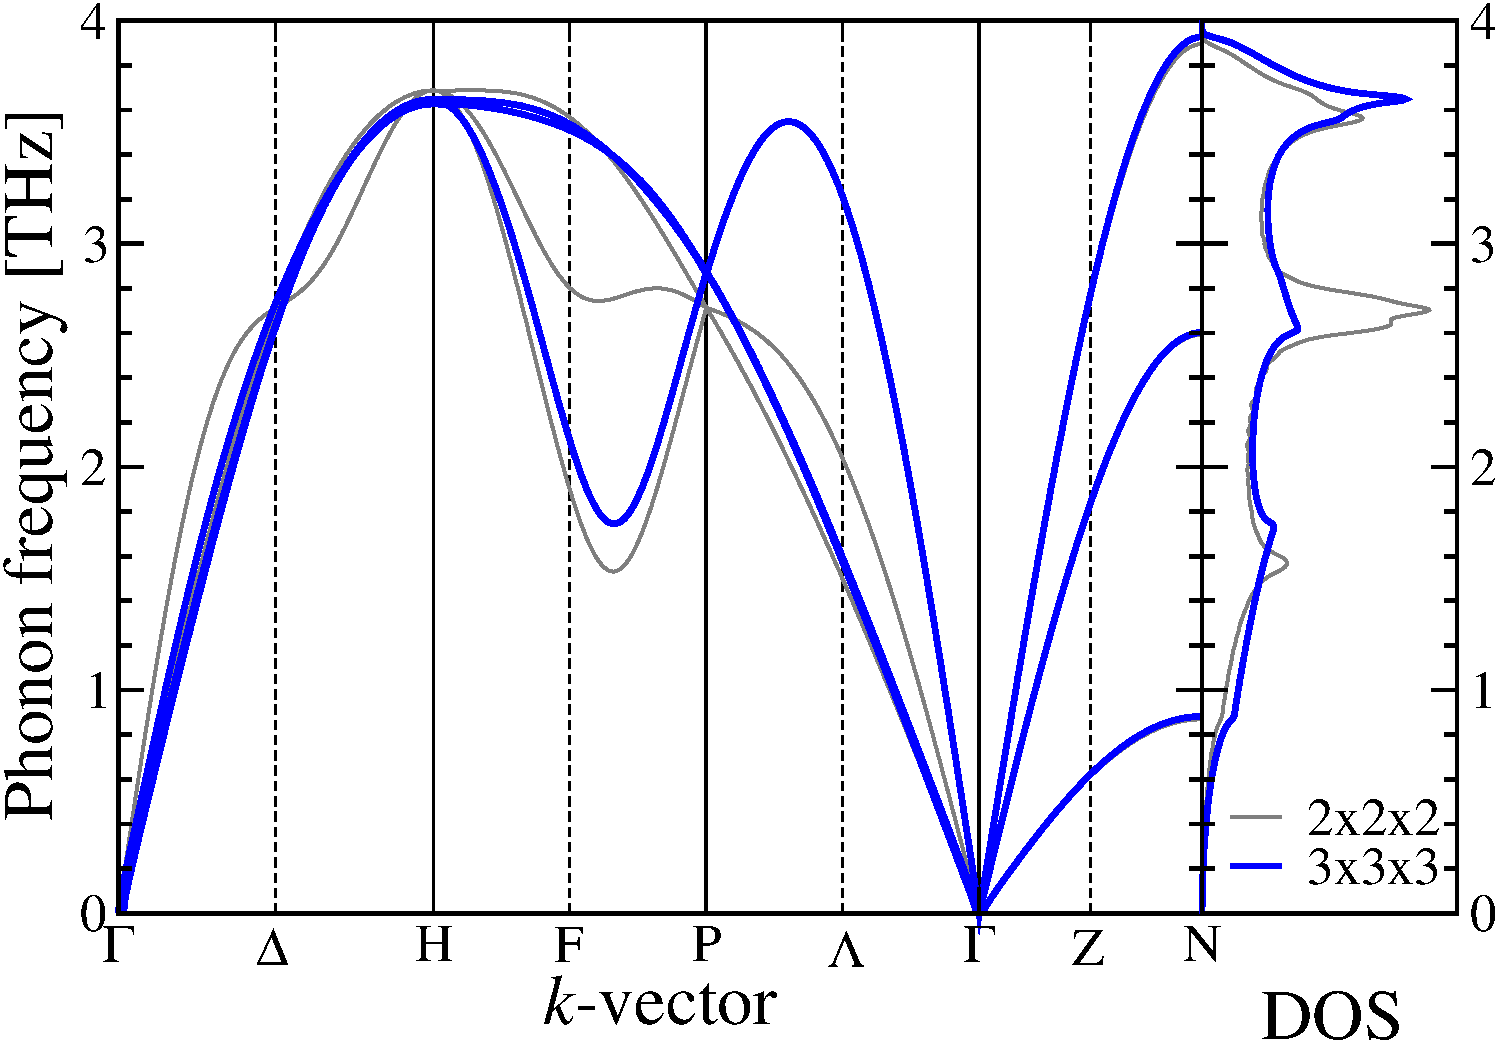
\includegraphics[height=7 cm]{Na_phonons}
\end{center}
\caption{The phonon band structure and density of states for
  sodium. Shown are calculations for a $3\times3\times3$ supercell in blue,
  with the $2\times2\times2$ results given in the thin grey lines for
  reference. The difference between these two plots shows that it is
  vital to converge phonon results with respect to supercell size.}
\label{sodium phonon figure}
\end{figure}

The user may also verify that the temptingly cheap setting 
\begin{verbatim}
  phonon supercell 2 2 2 
\end{verbatim}
does NOT give the correct phonon branch topology, which means that a
unit cell containing only 8 atoms is (not totally unexpectedly)
insufficient to descibe all the necessary interactions leading to the
proper phonon bands. For reference and tutorial purposes, we have
shown the phonon dispersion relation for this setting along with the
proper phonon dispersion in Fig. \ref{sodium phonon figure}. The user
may also verify that the $4\times4\times4$ supercell gives the same
result as those shown in blue, but he should be warned that this is a
numerically daunting task, as it involves 64-atom unit
cells. 



